The efficacy of the program was dependent on its ability to coordinate users and ensure that they were able to work together to generate the final instructions.
Thus, it was necessary to not only design an effective workflow, but to also make sure that the program implementation was easy to understand, robust, and close to the theoretical workflow.

\section{Workflow}
Turkomatic ran into difficulties in organizing the workflow. 
Their system was unable to coordinate workflows, in no small part due to the complexity of the algorithm.
Their algorithm used recursive workflow partitioning, and allowed for complex sub-task creation.
This led to significant difference of opinion between users, and little consensus was obtained without the use of a single task evaluator who would oversee the task (also known as ``derailment'' \cite{kulkarni2012collaboratively}.

To combat this problem, Canned Mentorship utilizes an iterative, chronological workflow.

\subsection{Greedy Instruction Addition}
Taking the opposite mentality, CannedMentorship uses a very simple task generating algorithm, with no explicit task subdivision or branching.
The system simply asks users to create steps in sequence, from beginning to end, in order.
Each step is completed in order, with the latter steps coming directly after former steps chronologically. 

\section{Implementation and Webapp details}
Our project began by creating a small webapp which coordinated the instruction generating process.
This program, also dubbed ``Canned Mentorship,'' consisted of two separate programs:

\begin{enumerate}
	\item a website interface for coordinating working users
	\item a back-end AI script for classifying answers and removing redundant inputs
\end{enumerate}

\section{System Implementation}

\subsection{The Webapp}
The webapp was a program written using Python Flask and was hosted on Heroku webapps. 
It was designed as a lightweight, simple system which hosted the users for the duration of the task and also coordinated their actions.

\begin{figure}[h]
	\begin{center}
		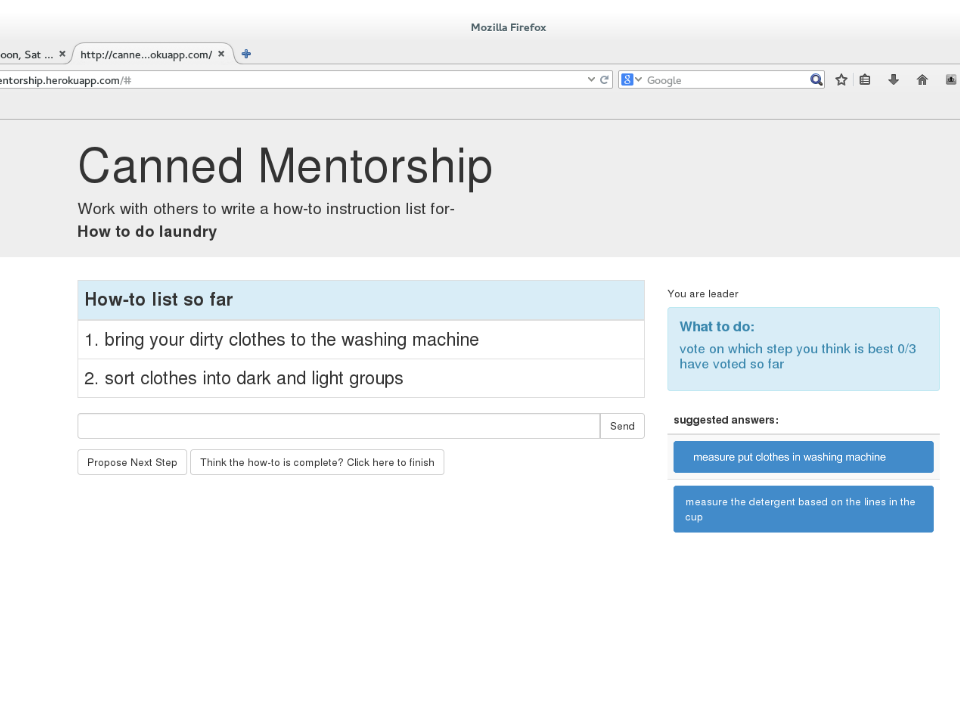
\includegraphics[width=0.48\textwidth]{figures/cmInterface2.png}
		\caption{Rejection sampling was also considered as a placement mechanism.}
		\label{fig:rejection_sampling_placement}
	\end{center}
\end{figure}

As noted earlier, Heroku was chosen as the host location for the webapp ...add more stuff later...



%webapp description
%theory
%need for multiple users: john's differences
%workflow
%implementation

%ai backend
%interface with program
%parameters
	%reasons for choosing
%flow
%
\begin{comment}
\begin{figure}[h]
	\begin{center}
		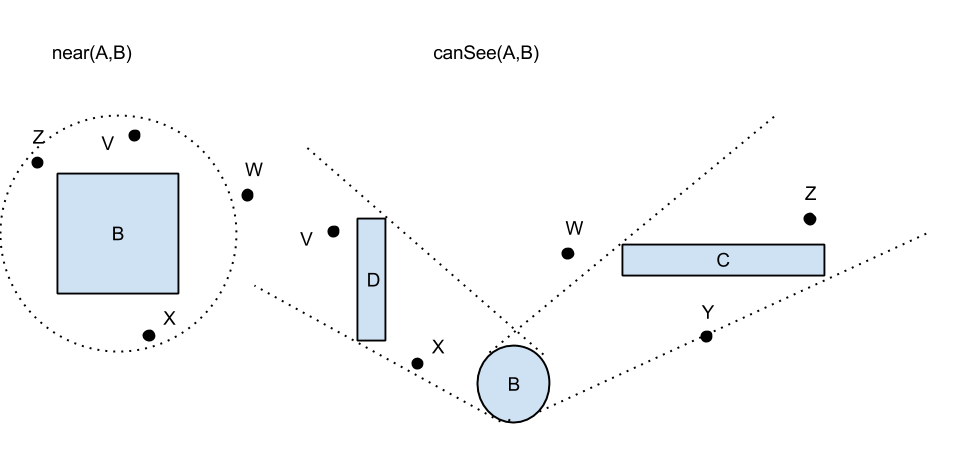
\includegraphics[width=0.48\textwidth]{figures/rejection_sampling_placement.png}
	\caption{Rejection sampling was also considered as a placement mechanism.}
	\label{fig:rejection_sampling_placement}
	\end{center}
\end{figure}
\end{comment}